Once a set of solvers is created, the last stage is to connect them to each other. Up to this point, solvers are disconnected, but they are ready to establish the communication. \posl{} provides tools  to the user to easily define cooperative strategies based on communication jacks and outlets. The pool of (concrete) connected solvers to be executed in parallel to solve a problem is called a \INTROsoset{}. 

%In the following we present two important concepts necessary to formalize \INTROcommoper.

\begin{definition}\label{def:comm_jack}
{\bf Communication Jack} Let $\mathcal{S}$ be a solver and a module $\mathcal{M}$. Then the operation $\mathcal{S}\cdot\mathcal{M}$ opens an outgoing connection from the solver $\mathcal{S}$, sending either 
\begin{inparaenum}[a)]
	\item the output of $\mathcal{M}$, if a sending data operator is applied to $\mathcal{M}$, as presented in Definition~\ref{op:osend}, or
	\item $\mathcal{M}$ itself, if a sending module operator is applied to $\mathcal{M}$, as presented in Definition~\ref{op:msend}.
\end{inparaenum}
\end{definition} 

\begin{definition}\label{def:comm_outlet}
{\bf Communication Outlet} Let $\mathcal{S}$ be a solver and a \opch{} $\mathcal{CM}$. Then, the operation $\mathcal{S}\cdot\mathcal{CM}$ opens an ingoing connection to the solver $\mathcal{S}$, receiving either 
\begin{inparaenum}[a)]
	\item the output of some \om{}, if $\mathcal{CM}$ is a \dopch{}, or
	\item a \om{}, if $\mathcal{CM}$ is an \oopch.
\end{inparaenum}
\end{definition} 

\separation

The communication is established by following the following rules guideline:
\begin{enumerate}%\begin{inparaenum}
	\item Each time a solver sends any kind of information by using a {\it sending} operator, it creates a \INTROjack.
	\item Each time a solver defines a \opch, it creates a \INTROoutlet. 
	\item Solvers can be connected to each other by linking \jacks{} to \outlets.
\end{enumerate} %\end{inparaenum}

%With the operator $(\cdot)$ we can have access to \oms{} sending information and to the \opch's names in a solver. 
%For example: $Solver_0\cdot \mathcal{M}$ provides access to the \om{} $\mathcal{M}$ in $Solver_0$ if and only if it is affected by a {\it sending} operator, and $Solver_1\cdot CM$ provides access to the \opch{} $CM$ in $Solver_1$.

Following, we define \textit{connection operators} that \posl{} provides.

\begin{definition}\label{op_conn:1to1}
\onetoone {\bf Connection One-to-One Operator} Let 
\begin{enumerate}
\item $\mathcal{J} = \left[\mathcal{S}_0\cdot \mathcal{M}_0, \mathcal{S}_1\cdot \mathcal{M}_1,\dots, \mathcal{S}_{N-1}\cdot \mathcal{M}_{N-1}\right]$ be the list of \jacks, and
\item $\mathcal{O} = \left[\mathcal{Z}_0\cdot \mathcal{CM}_0, \mathcal{Z}_1\cdot \mathcal{CM}_1,\dots, \mathcal{Z}_{N-1}\cdot \mathcal{CM}_{N-1}\right]$ be the list of \outlets{}
\end{enumerate} Then the operation 
\[
\mathcal{J} \onetoonesep \mathcal{O}
\]
connects each \jack{} $\mathcal{S}_i\cdot \mathcal{M}_i \in \mathcal{J}$ with the corresponding \outlet{} $\mathcal{Z}_i\cdot \mathcal{CM}_i \in \mathcal{O}$, $\forall\textbf{ }0 \leq i \leq N-1$ (see Figure~\ref{subfig:comm_simple}).
\end{definition}

\separation

\begin{definition}\label{op_conn:1ton}
\oneton {\bf Connection One-to-N Operator} Let 
\begin{enumerate} 
\item $\mathcal{J} = \left[\mathcal{S}_0\cdot \mathcal{M}_0, \mathcal{S}_1\cdot \mathcal{M}_1,\dots, \mathcal{S}_{N-1}\cdot \mathcal{M}_{N-1}\right]$ be the list of \jacks, and 
\item $\mathcal{O} = \left[\mathcal{Z}_0\cdot \mathcal{CM}_0, \mathcal{Z}_1\cdot \mathcal{CM}_1,\dots, \mathcal{Z}_{M-1}\cdot \mathcal{CM}_{M-1}\right]$ be the list of \outlets{} 
\end{enumerate} Then the operation 
\[
\mathcal{J} \onetonsep \mathcal{O}
\]
connects each \jack{} $\mathcal{S}_i\cdot \mathcal{M}_i \in \mathcal{J}$ with every \outlet{} $\mathcal{Z}_j\cdot \mathcal{CM}_j \in \mathcal{O}$, $\forall\textbf{ }0 \leq i \leq N-1$ and $0 \leq j \leq M-1$ (see Figure~\ref{subfig:comm_diff}).
\end{definition}

\separation

\begin{definition}\label{op_conn:ring}
\ring {\bf Connection Ring Operator} Let 
\begin{enumerate} 
\item $\mathcal{J} = \left[\mathcal{S}_0\cdot \mathcal{M}_0, \mathcal{S}_1\cdot \mathcal{M}_1,\dots, \mathcal{S}_{N-1}\cdot \mathcal{M}_{N-1}\right]$ be the list of \jacks, and 
\item $\mathcal{O} = \left[\mathcal{S}_0\cdot \mathcal{CM}_0, \mathcal{S}_1\cdot \mathcal{CM}_1,\dots, \mathcal{S}_{N-1}\cdot \mathcal{CM}_{N-1}\right]$ be the list of \outlets{} 
\end{enumerate} Then the operation 
\[
\mathcal{J} \ringsep \mathcal{O}
\]
connects each \jack{} $\mathcal{S}_i\cdot \mathcal{M}_i \in \mathcal{J}$ with the corresponding \outlet{} $\mathcal{Z}_{(i+1)\%N}\cdot \mathcal{CM}_{(i+1)\%N} \in \mathcal{O}$, $\forall 0 \leq i \leq N-1$  (see Figure~\ref{subfig:comm_ring}).
\end{definition}

\separation

\posl{} also allows to declare non-communicating solvers to be executed in parallel, declaring only the list of solver names:
\[
\left[\mathcal{S}_0, \mathcal{S}_1, \dots, \mathcal{S}_{N-1}\right]
\]

\begin{figure}[h]
\centering
\subfloat[][Communication 1 to 1]{
	\label{subfig:comm_simple}
	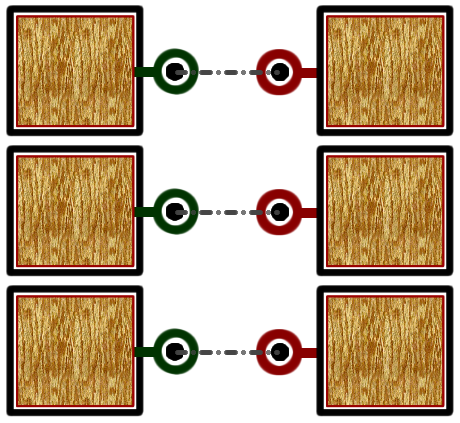
\includegraphics[width=0.25\textwidth]{comm_11.png}
}
\hspace{0.05\textwidth}%
\subfloat[][Communication 1 to N]{%
	\label{subfig:comm_diff}
	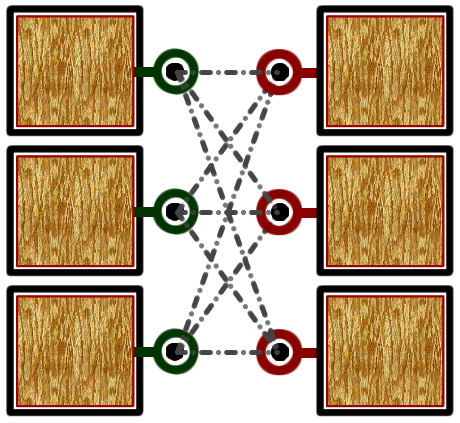
\includegraphics[width=0.25\textwidth]{comm_1n.png}
}
\hspace{0.05\textwidth}%
\subfloat[][Cyclic communication]{%
	\label{subfig:comm_ring}
	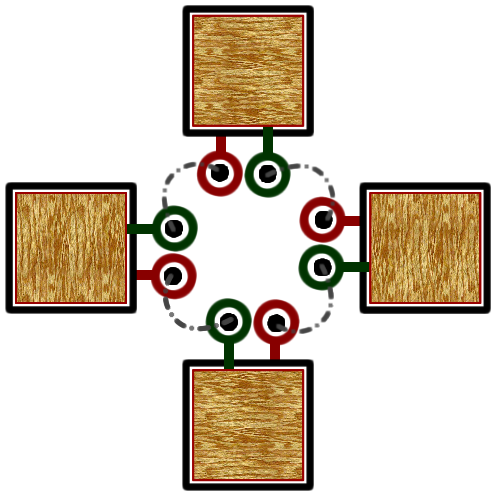
\includegraphics[width=0.25\textwidth]{comm_ring2.png}
}
\caption[]{Graphic representation of communication operators}
\label{fig:comm}
\end{figure}

\poslexample{These operators can be combined beteewn themself to contruct any kind of \comstr. Figure~\ref{fig:ex:comb} shows a simple example combining solvers doubly connected and non connected solvers. Assuming that all solvers $S_i, i\in[1..5]$ have a module $\mathcal{M}$ sent by a send operator, and a \opch{} $\mathcal{CM}$, the corresponding code is the following:
\begin{gather*}
\left[\mathcal{S}_1\cdot\mathcal{M}, \mathcal{S}_2\cdot\mathcal{M}, \mathcal{S}_{3}\cdot\mathcal{M}\right] \onetonsep \left[\mathcal{S}_4\cdot\mathcal{CM}, \mathcal{S}_5\cdot\mathcal{CM}\right]\\
\left[\mathcal{S}_4\cdot\mathcal{M}, \mathcal{S}_5\cdot\mathcal{M}\right] \onetoonesep \left[\mathcal{S}_1\cdot\mathcal{CM}, \mathcal{S}_{3}\cdot\mathcal{CM}\right]\\
\left[\mathcal{S}_6\right]\\
\left[\mathcal{S}_7\right]
\end{gather*}
}

\begin{figure}[h]
\centering
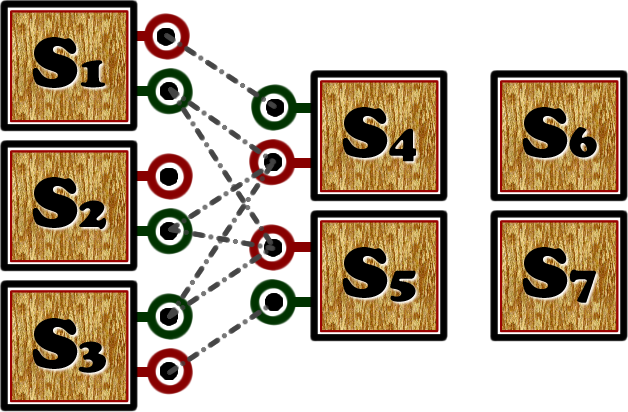
\includegraphics[width=0.35\textwidth]{ex_comb.png}
\caption[]{Graphic representation of communication operators}
\label{fig:ex:comb}
\end{figure}

\separation

%When we apply a connection operator $\circled{op}$ between a \jacks{} list $\mathcal{J}$ and a \outlets{} list $\mathcal{O}$, internally we are assigning an \textit{computation unit} (typically a thread) to each solver that we declare in each list. This assignment receives the name of \textit{Solver Scheduling}. Before running the \soset{}, this \textit{computation unit} is just an integer $\tau \in [0..N]$ identifying uniquely each of the solvers. When the \soset{} is launched, the solver with the identifier $\tau$ runs inside the computation unit $\tau$. This identifier assignation remains independent of the real availability of resources of computation. It just takes into account the user declaration. This means that, if the user declares 30 solvers (15 senders and 15 receivers) and the \soset{} is launched using 20 cores, only the first 20 solvers will be executed, and in consequence, there will be 10 solvers sending information to nowhere. Users should take this into account when declaring the \soset.

The connection process depends on the applied connection operator. In each case the goal is to assign, to the sending operator ($\senddataop{.}$ or $\sendmoduleop{.}$) inside the \as{}, the identifier of the solver (or solvers, depending on the connection operator) where the information will be sent. Algorithm~\ref{algo:connecting} presents the connection process.

\incmargin{1.4em}
\linesnumbered
\begin{algorithm}[H]
\dontprintsemicolon
\SetLine
\SetKwFor{While}{while}{do}{end}
\SetKwData{Jacks}{$\mathcal{J}$}
\SetKwData{Outlets}{$\mathcal{O}$}
\SetKwData{SS}{$S$}
\SetKwData{SSjack}{$S_{jack}$}
\SetKwData{RR}{$R$}
\SetKwData{RRoutlet}{$R_{outlet}$}
\SetKwData{RRid}{$R_{id}$}
\SetKwFunction{GetSolver}{GetSolverFromConnector}
\SetKwFunction{GetNext}{GetNext}
\SetKwFunction{Sched}{Schedule}
\SetKwFunction{Root}{root}
\SetKwFunction{Connect}{Connect}
\SetKwInOut{Input}{input}
\SetKwInOut{Output}{output}
\SetKw{KwTo}{int}

\Input{\Jacks list of \jacks{}, \\ \Outlets list of \outlets}
%\Output{\Q = $\left\{Q_i\right\}_{i=1\dots K}$: $K$ subsets of \Uni}
%\BlankLine
\While{no available jacks or outlets remain}{ %\nllabel{paso_condicion}
	\SSjack	$\leftarrow$ \GetNext{\Jacks}\;
	\RRoutlet $\leftarrow$ \GetNext{\Outlets}\;
	\SS $\leftarrow$ \GetSolver{\SSjack}\;	
	\RR $\leftarrow$ \GetSolver{\RRoutlet}\;
	%\Sched{\SS}\;
	%\RRid $\leftarrow$ \Sched{\RR}\;
	\Connect{\Root{\SS},\SSjack, \RR} %\RRid} %\label{step2} \tcc{It also removes the returned element}
}
\caption{Connection main algorithm}\label{algo:connecting}
\end{algorithm}

In Algorithm~\ref{algo:connecting}:
\begin{itemize}
\item \texttt{GetNext($\dots$)} returns the next available solver-jack (or solver-outlet) in the list, depending on the connection operator, e.g., for the connection operator One-to-N, each \jack{} in $\mathcal{J}$ must be connected with each \outlet{} in $\mathcal{O}$.
\item \texttt{GetSolverFromConnector($\dots$)} returns the solver name given a connector declaration.
%\item \texttt{Schedule($\dots$)} schedules a solver and returns its identifier.
\item \texttt{Root($\dots$)} returns the {\it root} \cm{} of a solver.
\item \texttt{Connect($\dots$)} %is presented in Algorithm~\ref{algo:connect}. It 
searches the \om{} $S_{jack}$ recursively inside the {\it root} \cm{} of $S$ and places the identifier $R_{id}$ into its list of destination solvers.
\end{itemize}

\poslexample{Let us suppose that we have declared two solvers $S$ and $Z$, both implementing the \as{} in Algorithm~\ref{algo:as_example}, so they can be either sender or receiver. The following code connects them using the operator {\bf 1~to~N}:
$$\left[S\cdot A\right] \onetonsep \left[Z\cdot C.M.\right]$$
If the operator {\bf 1~to~N} is used with only with one solver in each list, the operation is equivalent to applying the operator {\bf 1~to~1}. However, to obtain a communication strategy like the one showed in Figure~\ref{subfig:comm_diff}, six solvers (three senders and three receivers) have to be declared to be able to apply the following operation:
$$\left[S_1\cdot A, S_2\cdot A, S_3\cdot A\right]\onetonsep \left[Z_1\cdot C.M., Z_2\cdot C.M., Z_3\cdot C.M.\right]$$
\posl{} provides a mechanism to make this easier, through two {\it syntactic sugars} explained below.
}

%\subsection{Solver namespace expansion}
\separation

One of the goals of \posl{} is to provide a way to declare sets of solvers to be executed in parallel easily. For that reason, \posl{} provides two syntactic sugars %forms of namespace expansion, 
in order to create sets of solvers using already declared ones:
\begin{enumerate}
\item Using an integer to denote how many times a solver name will appear in the declaration.
\item Using an integer to denote how many times the connection will be repeated in the declaration.
\end{enumerate}

The following example explains clearly these syntactic sugars:

%\textbf{Solver name expansion - } Uses an integer $K$ to denote how many times the solver name $S$ will appear in the declaration. $\left[\dots S_i\cdot\mathcal{M}(K),\dots\right]$ expands as $\left[\dots S_i\cdot\mathcal{M}, S_i^2\cdot\mathcal{M},\dots S_i^K\cdot\mathcal{M}\dots\right]$\\
%and all new solvers $S_i^j, j\in [2..K]$ are created using the same solver declaration of solver $S_i$.

%\textbf{Connection declaration expansion - } Uses an integer $K$ to denote how many times the connection will be repeated in the declaration. Let 
%\begin{inparaenum}[a)]
%\item $\left[\mathcal{S}_1\cdot\mathcal{M}_1,\dots,\mathcal{S}_{N}\cdot\mathcal{M}_{N}\right]$ and 
%\item $\left[\mathcal{R}_1\cdot\mathcal{CM}_1,\dots,\mathcal{R}_{M}\cdot\mathcal{CM}_{M}\right]$ be the list of \jacks{} and \outlets, respectively, and
%\item $\circled{op}$ a connection operator.
%\end{inparaenum} Then $$\left[\mathcal{S}_1\cdot\mathcal{M}_1,\dots,\mathcal{S}_{N}\cdot\mathcal{M}_{N}\right] \poslop{op} \left[\mathcal{R}_1\cdot\mathcal{CM}_1,\dots,\mathcal{R}_{M}\cdot\mathcal{CM}_{M}\right]K$$ expands as
%
%\begin{align*}
%\left[\mathcal{S}_1\cdot\mathcal{M}_1,\dots,\mathcal{S}_{N}\cdot\mathcal{M}_{N}\right] &\poslop{op} \left[\mathcal{R}_1\cdot\mathcal{CM}_1,\dots,\mathcal{R}_{M}\cdot\mathcal{CM}_{M}\right]\\
%\left[\mathcal{S}_1^2\cdot\mathcal{M}_1,\dots,\mathcal{S}_{N}^2\cdot\mathcal{M}_{N}\right] &\poslop{op} \left[\mathcal{R}_1^2\cdot\mathcal{CM}_1,\dots,\mathcal{R}_{M}^2\cdot\mathcal{CM}_{M}\right]\\
%&\dots\\
%\left[\mathcal{S}_1^K\cdot\mathcal{M}_1,\dots,\mathcal{S}_{N}^K\cdot\mathcal{M}_{N}\right] &\poslop{op} \left[\mathcal{R}_1^K\cdot\mathcal{CM}_1,\dots,\mathcal{R}_{M}^K\cdot\mathcal{CM}_{M}\right]\\
%\end{align*}
%and all new solvers $S_i^k, i\in[1..N]$ and $R_j^k,j\in [1..M]$, $k\in[2..K]$, are created using the same solver declaration of solvers $S_i$ and $R_j$, respectively.

\poslexample{Suppose that I have created  solvers $S$ and $Z$ mentioned in the previews example. As a communication strategy, I want to connect them through the operator {\bf 1~to~N}, using $S$ as sender and $Z$ as receiver. Then,  %using \textbf{namespace expansions}, 
we need to declare how many solvers I want to connect. Algorithm~\ref{algo:comm_str_ex} shows the desired communication strategy. Notice in this example that the connection operation is affected also by the number $2$ at the end of the line. %, as {\bf connection declaration expansion}. 
In that sense, and supposing that 12 units of computation are available, a \soset{} working on parallel following the topology described in Figure~\ref{fig:ex_conn} can be obtained.}

\begin{algorithm}[H]
\dontprintsemicolon
\SetNoline
%\myproc{
[ S$\cdot A$ (3) ] $\onetonsep$ [ Z$\cdot C.M.$ (3) ] 2 ;
\caption{A communication strategy}\label{algo:comm_str_ex}
\end{algorithm}

\begin{figure}[h]
	\centering	
	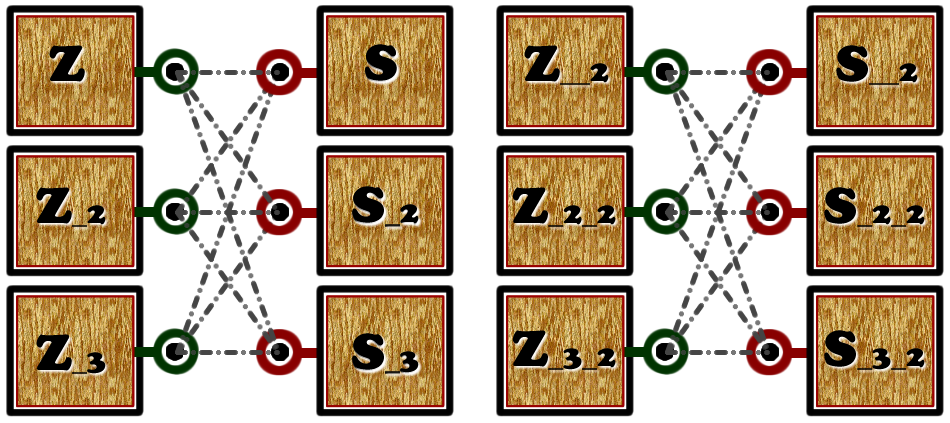
\includegraphics[width=0.6\linewidth]{ex_top.png}
	\caption{An example of connection strategy for 12 units of computation}\label{fig:ex_conn}
\end{figure}